\documentclass[
  captions=tableheading,
  bibliography=totoc, 
  titepage=firstiscover,
]{scrartcl}

\usepackage{blindtext} %neuer input

\usepackage{longtable} % Tabellen über mehrere Seiten

\usepackage[utf8]{inputenc} %neuer input

\usepackage{scrhack}

\usepackage[aux]{rerunfilecheck} %Warnung falls nochmal kompiliert werden muss

\usepackage{fontspec} %Fonteinstellungen

\recalctypearea{}

\usepackage[main=ngerman]{babel} %deutsche Spracheinstellung

\usepackage{ragged2e} %neuer input

\usepackage{amsmath, nccmath}

\usepackage{amssymb} %viele mathe Symbole

\usepackage{mathtools} %Erweiterungen für amsmath


\DeclarePairedDelimiter{\abs}{\lvert}{\rvert}
\DeclarePairedDelimiter{\norm}{\lVert}{\rVert}

\DeclarePairedDelimiter{\bra}{\langle}{\rvert}
\DeclarePairedDelimiter{\ket}{\lvert}{\rangle}

\DeclarePairedDelimiterX{\braket}[2]{\langle}{\rangle}{
#1 \delimsize| #2
}

\NewDocumentCommand \dif {m}
{
\mathinner{\symup{d} #1}
}


\usepackage[
  math-style=ISO,
  bold-style=ISO,
  sans-style=italic,
  nabla=upright,
  partial=upright,
  warnings-off={
    mathtools-colon,
    mathtools-overbracket,
  },
]{unicode-math}

\setmathfont{Latin Modern Math}
\setmathfont{XITS Math}[range={scr, bfscr}]
\setmathfont{XITS Math}[range={cal, bfcal}, StylisticSet=1]


\usepackage[
  locale=DE,
  separate-uncertainty=true,
  per-mode=reciprocal,
  output-decimal-marker={,},
]{siunitx}

\usepackage[autostyle]{csquotes} %richtige Anführungszeichen

\usepackage{xfrac}

\usepackage{float}

\floatplacement{figure}{htbp}

\floatplacement{table}{htbp}

\usepackage[ %floats innerhalb einer section halten
  section,   %floats innerhalb er section halten
  below,     %unterhalb der Section aber auf der selben Seite ist ok
]{placeins}

\usepackage[
  labelfont=bf,
  font=small,
  width=0.9\textwidth,
]{caption}

\usepackage{subcaption} %subfigure, subtable, subref

\usepackage{graphicx}

\usepackage{grffile}

\usepackage{booktabs}

\usepackage{microtype} %Verbesserungen am Schriftbild

\usepackage[
backend=biber,
]{biblatex}

\addbibresource{../lit.bib}

\usepackage[ %Hyperlinks im Dokument
  german,
  unicode,
  pdfusetitle,
  pdfcreator={},
  pdfproducer={},
]{hyperref}

\usepackage{bookmark}

\usepackage[shortcuts]{extdash}

%\usepackage{warpcol}

\usepackage{physics}
\allowdisplaybreaks

\begin{document}
    \title{Physik IV Übungsblatt 12}
    \author{  
    Tobias Rücker\\
    \texorpdfstring{\href{mailto:tobias.ruecker@tu-dortmund.de}{tobias.ruecker@tu-dortmund.de}
    \and}{,} 
    Paul Störbrock\\
    \texorpdfstring{\href{mailto:paul.stoerbrock@tu-dortmund.de}{paul.stoerbrock@tu-dortmund.de}}{}
    }
\maketitle
\center{\Large Abgabegruppe: \textbf{4H}}
\thispagestyle{empty}

\newpage
\tableofcontents
\thispagestyle{empty}
\newpage

\setcounter{page}{1}

\section{Aufgabe 1}
\begin{figure}[H]
    \centering
    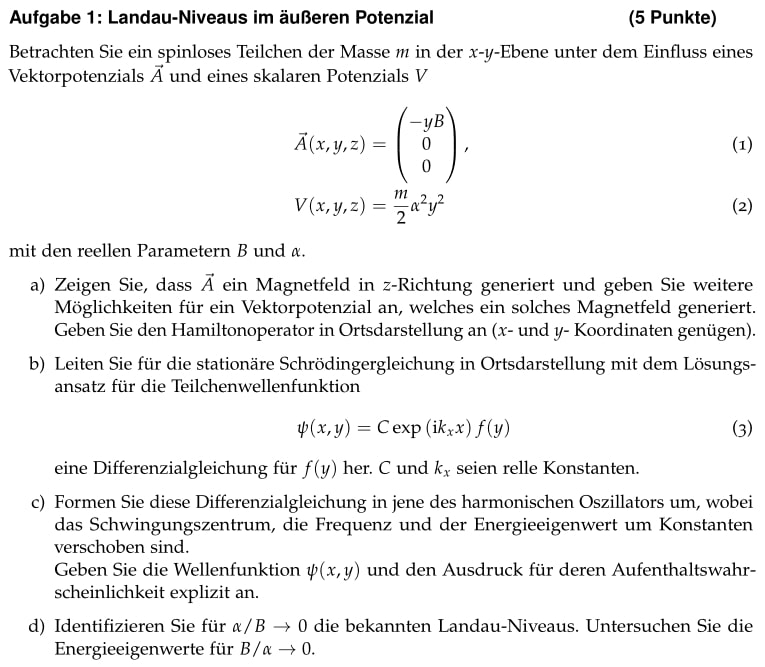
\includegraphics[width=\textwidth]{images/Aufgabe1.jpg}
\end{figure}

\subsection{a)}

    \begin{align}
        \vec{\nabla} \times \vec{A} &= \vec{B}\\
        \vec{\nabla} \times
        \begin{pmatrix}
            -yB\\
            0\\
            0
        \end{pmatrix}
        &= \begin{pmatrix}
            0\\
            0\\
            B
        \end{pmatrix}
        \intertext{
            \flushleft{Ein\;}\justifying weiteres Vektorpotential mit gleichem B-Feld wäre:
        }
        \vec{A} &= \begin{pmatrix}
            -yB\\
            0\\
            0
        \end{pmatrix} + \vec{\nabla}f
        \intertext{
            \flushleft{wobei\;}\justifying $\nabla f$ ein beliebiges Gradientenfeld mit $rot(\nabla f)=0$ ist.
        }
        \hat{H} &= \frac{1}{2m} \left( \hat{\vec{p}} - q\vec{A} \right)^2 + \hat{V}\\
        &= \frac{1}{2m} \left( \begin{pmatrix}
            \hat{p}_x\\
            \hat{p}_y\\
            0
        \end{pmatrix} -q \begin{pmatrix}
            -\hat{y}B\\
            0\\
            0
        \end{pmatrix} \right)^2 + \frac{m}{2} \alpha^2 \hat{y}^2\\
        &= \frac{1}{2m} \left( \hat{p}_x \hat{y}qB \right)^2 + \frac{1}{2m} \hat{p}_y^2 + \frac{m}{2} \alpha^2 \hat{y}^2\\
        &= \frac{1}{2m} \hat{p}_x^2 + \frac{qB}{m} \hat{y} \hat{p}_x + \frac{1}{2m} \hat{p}_y^2 + \left( \frac{q^2 B^2}{2m} + \frac{m}{2}\alpha^2 \right) \hat{y}^2
    \end{align}

\subsection{b)}

    \begin{align}
        &\hat{H}\Psi = \hat{E}\Psi\\
        &\left( \frac{1}{2m} \left( -\hbar^2 \frac{\partial^2}{\partial x^2} \right) -i \frac{qB\hbar}{m} y \frac{\partial}{\partial x} - \frac{\hbar^2}{2m} \frac{\partial^2}{\partial y^2} + \left( \frac{q^2 B^2}{2m} + \frac{m}{2} \alpha^2 \right) y^2 \right) C\exp\left( ik_x x \right) f(y) = E \cdot C\exp\left( ik_x x \right) f(y)\\
        &-\frac{\hbar^2 k_x^2}{2m} f(y) - \frac{\hbar^2}{2m} f\prime\prime(y) + \left( \frac{q^2 B^2}{2m} + \frac{m}{2} \alpha^2 \right) y^2 f(y) + \frac{k_x q B \hbar}{m} yf(y) = Ef(y)\\
        \Leftrightarrow &-\frac{\hbar^2}{2m} f\prime\prime (y) = \left( - \left( \frac{q^2 B^2}{2m} + \frac{m}{2}\alpha^2 \right) y^2 - \frac{k_x q B \hbar}{m} y + \frac{\hbar^2 k_x^2}{2m} + E \right) f(y)
    \end{align}

\subsection{c)}

    \flushleft{Gesucht\;}\justifying wird eine DGL in der Form der eines harmonischen Oszillators
    \begin{align}
        &-\frac{\hbar^2}{2m} f\prime\prime(y) + \frac{1}{2} m \omega^2 y^2 f(y) = Ef(y)\\
        &-\frac{\hbar^2}{2m} f\prime\prime(y) = \left( - \left( \frac{q^2 B^2}{2m} + \frac{m}{2}\alpha^2 \right) y^2 - \frac{k_x q B \hbar}{m} y + \underbrace{\frac{\hbar^2 k_x^2}{2m} + E}_{C} \right) f(y)\\
        &-\frac{\hbar^2}{2m} f\prime\prime(y) = \left( - \left( \frac{q^2 B^2}{2m} + \frac{m}{2}\alpha^2 \right) y^2 - \frac{k_x q B \hbar}{m} y + C \right) f(y)\\
        &= \left( - \underbrace{\left( \overbrace{\frac{q^2 B^2}{2m}}^{\omega^2} + \frac{m}{2}\alpha^2 \right)}_{a} y^2 - 2\underbrace{\frac{k_x q B \hbar}{m^2}}_{b} y + C \right) f(y)\\
        &= \left(-\frac{1}{2}m a \left( y^2 + \frac{2b}{a} y + \frac{b^2}{a^2} - \frac{b^2}{a^2} \right) \right) f(y)\\
        &= \left(-\frac{1}{2}m \underbrace{a}_{\omega^2} \left( \underbrace{y + \frac{b}{a}}_{\tilde{y}} \right)^2 + \underbrace{\frac{1}{2} m \frac{b^2}{a} + C}_{\tilde{E}} \right) f(y) \qquad \text{mit}\; a=\omega^2+\alpha^2\\
        &-\frac{\hbar^2}{2m}f\prime\prime(y) + \frac{1}{2} m \tilde{\omega}^2 \tilde{y}^2 f(y) = \tilde{E}f(y)
        \intertext{
            \flushleft{Die\;}\justifying allgemeine Lösung des harm. Oszillators lautet:
        }
        f_n(y) &= \left( 2^n n! \sqrt{\pi} y_0 \right)^{-\sfrac{1}{2}} \exp\left( -\frac{\left(\frac{\tilde{y}}{y_0}\right)^2}{2} \right) H_n \left( \frac{\tilde{y}}{y_0} \right) \qquad \text{mit}\; y_0 = \left( \frac{\hbar \tilde{\omega}}{m} \right)^{\sfrac{1}{2}}\\
        \Psi_n(x,y) &= \left( 2^n n! \sqrt{\pi} y_0 \right)^{-\sfrac{1}{2}} \exp\left( -\frac{\left(\frac{\tilde{y}}{y_0}\right)^2}{2} \right) H_n \left( \frac{\tilde{y}}{y_0} \right) \cdot C\exp\left( ik_x x \right)\\
        \abs{\Psi_n(x,y)}^2 &= \Psi_n^* \Psi_n \\
        &= 2^n n! \sqrt{\pi} y_0 \exp\left( -\left(\frac{\tilde{y}}{y_0}\right)^2 \right) C^2
        \intertext{
            \flushleft{$H_n$\;}\justifying stehen orthogonal zueinander.
        }
    \end{align}

\subsection{d)}

    \begin{align}
        E_n &= \hbar \tilde{\omega} \left( n+\frac{1}{2} \right)\\
        &= \hbar \sqrt{ \omega^2 + \alpha^2} \left( n+\frac{1}{2} \right) \qquad \text{mit}\; \omega^2 = \frac{q^2 B^2}{m^2}\\
        &= \hbar \sqrt{ \frac{q^2 B^2}{m^2} + \alpha^2} \left( n+\frac{1}{2} \right)\\
        &= \hbar \alpha \sqrt{\frac{q^2}{m^2} \underbrace{\frac{B^2}{\alpha^2}}_{\to 0} + 1}\\
        E_n &= \hbar \alpha \left( n+\frac{1}{2} \right) 
        \intertext{
            \flushleft{Im\;}\justifying Falle, dass $\sfrac{B}{\alpha} \to 0$ geht, bildet $\alpha$ unsere Eigenfrequenz.\\
            Landau-Niveaus:
        }
        E_n &= \hbar B \sqrt{\frac{q^2}{m^2} + \underbrace{\frac{\alpha^2}{B^2}}_{\to 0}} \left( n+\frac{1}{2} \right)\\
        &= \hbar \frac{Bq}{m} \left( n+\frac{1}{2} \right) 
    \end{align}

\section{Aufgabe 2}
\begin{figure}[H]
    \centering
    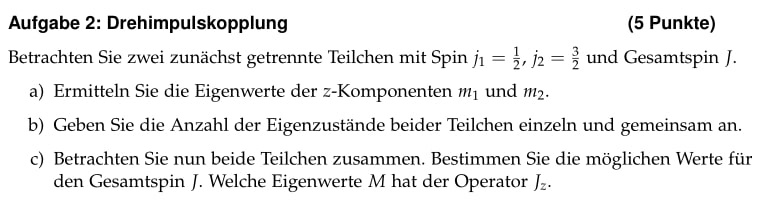
\includegraphics[width=\textwidth]{images/Aufgabe2a.jpg}
\end{figure}

\begin{figure}[H]
    \centering
    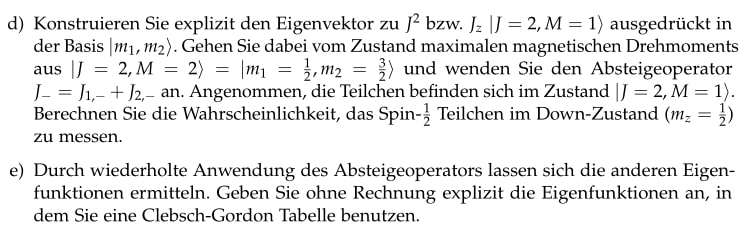
\includegraphics[width=\textwidth]{images/Aufgabe2b.jpg}
\end{figure}

\subsection{a)}

\subsection{b)}

\subsection{c)}

\subsection{d)}

\subsection{e)}

\section{Aufgabe 3}
\begin{figure}[H]
    \centering
    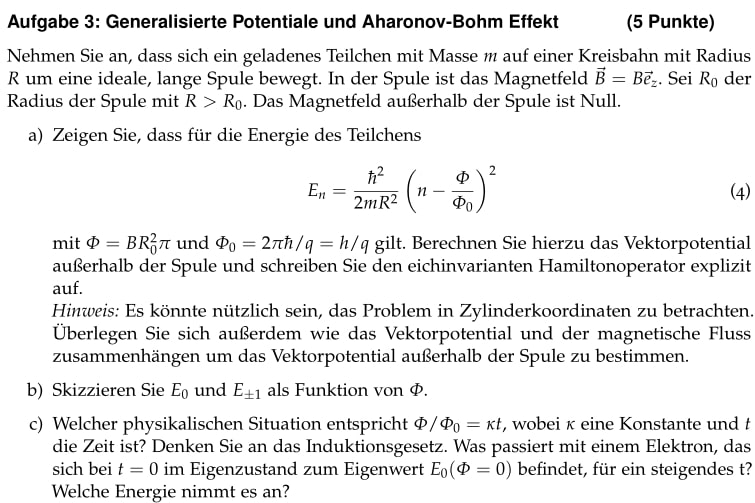
\includegraphics[width=\textwidth]{images/Aufgabe3.jpg}
\end{figure}

\subsection{a)}

\subsection{b)}

\subsection{c)}

\section{Aufgabe 4}
\begin{figure}[H]
    \centering
    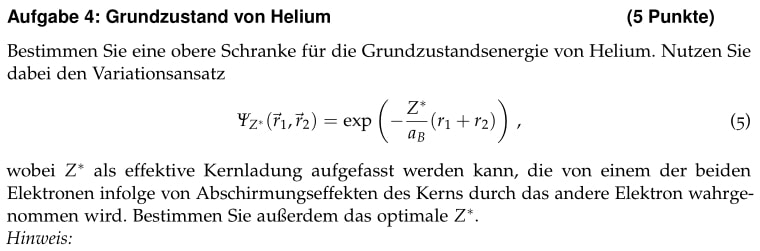
\includegraphics[width=\textwidth]{images/Aufgabe4a.jpg}
\end{figure}

\begin{figure}[H]
    \centering
    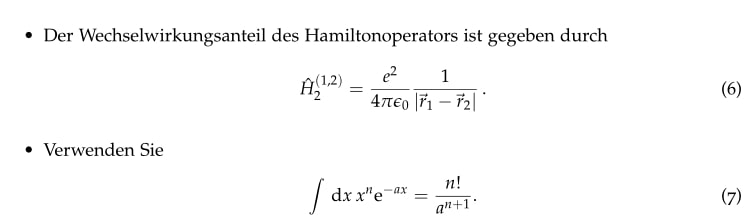
\includegraphics[width=\textwidth]{images/Aufgabe4b.jpg}
\end{figure}

    \flushleft{Gegeben\;}\justifying sind:\\
    Der Wechselwirkungsanteil des Hamiltonoperators
    \begin{align}
        \hat{H}_2^{(1,2)} &= \frac{e^2}{4\pi\epsilon_0}\frac{1}{\abs{\vec{r}_1-\vec{r}_2}}
        \intertext{
            \flushleft{Der\;}\justifying Variationsansatz
        }
        \Psi_{Z^*}(\vec{r}_1,\vec{r}_2) &= \exp\left( -\frac{Z}{a_B}(\vec{r}_1+\vec{r}_2) \right)
        \intertext{
            \flushleft{Und\;}\justifying Variationsansatz die Beziehung
        }
        \int \mathrm{d}x\; x^n e^{-\alpha x} &= \frac{n!}{a^{n+1}}
        \intertext{
            \flushleft{Normierung\;}\justifying Variationsansatz der Wellenfunktion:
        }
        \braket{\Psi_{Z^*}}{\Psi_{Z^*}} &= 16\pi^2 \int_{0}^{\infty} \int_{0}^{\infty} \mathrm{d}r_1\; \mathrm{d}r_2\; r_1^2 r_2^2 \exp\left( -\frac{Z}{a_B}(\vec{r}_1+\vec{r}_2) \right)\\
        &= \left[ 4\pi \int_{0}^{\infty} \mathrm{d}r\; r^2 \exp\left( \frac{2Z^*}{a_B}r \right) \right]^2\\
        &= \left[ 4\pi \cdot 2! \cdot \left( -\frac{a_B}{2Z^*} \right)^3 \right]^2\\
        &= \pi^2 \frac{a_B^6}{Z^{*6}}
    \end{align}
    \flushleft{Anschließend\;}\justifying wird das Funktional gebildet mit:
    \begin{align}
        &\bra{\Psi_{Z*}} \left( H_1^{(1)} + H_1^{(2)} \right) \ket{\Psi_{Z*}} \stackrel{H_1^{(1)}=H_1^{(2)}}{=} 2\bra{\Psi_{Z*}} H_1^{(2)} \ket{\Psi_{Z*}}\\
        &= 2\underbrace{\int \mathrm{d}^3r_1\; \exp\left( -\frac{2Z^*}{a_B}r_1 \right)}_{\frac{\pi a_B^3}{Z^{*^3}}} \int \mathrm{d}^3r_2\; \exp\left( -\frac{2Z^*}{a_B}r_2 \right) \left( -\frac{\hbar^2}{2m} \Delta_2 -\frac{2e^2}{4\pi\epsilon_0}\frac{1}{r_2} \right) \exp\left( -\frac{Z}{a_B}r_2 \right)\\
        &= \frac{\pi a_B^3}{Z^{*^3}}4\pi \int \mathrm{d}^3r_2\;r_2^2 \exp\left( -\frac{Z^*}{a_B}r_2 \right) \left( -\frac{\hbar^2}{2m} \left( \frac{\partial^2}{\partial r_2^2} + \frac{2}{r_2} \frac{\partial}{\partial r_2} \right) -\frac{2e^2}{4\pi\epsilon_0}\frac{1}{r_2}  \right) \exp\left( -\frac{Z}{a_B}r_2 \right)\\
        &= \frac{8\pi^2 a_B^3}{Z^{*^3}} \int \mathrm{d}^3r_2\;r_2^2 \exp\left( -\frac{2Z^*}{a_B}r_2 \right) \left( -\frac{\hbar^2}{2m} \left( \frac{Z^{*^2}}{a_B^2}r_2^2 - \frac{2Z^*}{a_B}r_2 \right) -\frac{2e^2 r^2}{4\pi\epsilon_0} \right)\\
        &= \frac{8\pi^2 a_B^3}{Z^{*^3}} \left( \frac{\hbar^2 a_B}{8m Z^*} - \frac{e^2 a_B^2}{8\pi \epsilon_0 Z^{*^2}} \right)\\
        &\boxed{E_R = \frac{e^2}{8\pi \epsilon_0 a_B},\;a_B = \frac{4\pi\hbar^2\epsilon_0}{me^2} \Rightarrow \frac{\hbar^2}{m} = \frac{a_B e^2}{4\pi \epsilon_0} = 2a_B^2 E_R}\\
        &= \frac{8\pi^2 a_B^3}{Z^{*^3}} \left( \frac{1}{4Z^*} - \frac{1}{Z^{*^2}} \right)\\
        \\
        &\frac{\bra{\Psi_{Z^*}}\left( H_1^{(1)} + H_1^{(2)} \right)\ket{\Psi_{Z^*}}}{\braket{\Psi_{Z^*}}{\Psi_{Z^*}}} = \frac{Z^{*^6}}{\pi^2 a_B^6} \frac{8\pi^2 a_B^2}{Z^{*^3}} E_R\left( \frac{1}{4Z^*} - \frac{1}{Z^{*^2}} \right)\\
        &= E_R \left( 2Z^{*^2} - 8Z^* \right)
        \intertext{
            \flushleft{Abschließend\;}\justifying wird das Wirkungsfunktional über die Störungstheorie 1. Ordnung bestimmt:
        }
        &\bra{\Psi_{Z*}} \left( H_2^{(1,2)} \right) \ket{\Psi_{Z*}} = \frac{e^2}{4\pi\epsilon_0} \int \int \mathrm{d}^3r_1 \mathrm{d}^3r_2\; \frac{\exp\left( -\frac{2Z^*}{a_B}(r_1+r_2) \right)}{\abs{r_1-r_2}}
        \intertext{
            \flushleft{Da\;}\justifying der Integrand in $r_1$ und $r_2$ symmetrisch ist, kann $r_2\geq r_1$ angenommen und als Faktor 2 an das Ergebnis multipliziert werden:    
        }
        &\boxed{\frac{e^2}{4\pi\epsilon_0} = 2a_BE_R}\\
        &= 8\pi a_BE_R \underbrace{\int \mathrm{d}^3r_1\; \exp\left( \frac{2Z^*}{a_B}r_1 \right)}_{Q} \underbrace{\int_{r_1}^{\infty} \mathrm{d}r_2\; r_2^2 \exp\left( -\frac{2Z^*}{a_B}r_2 \right)}_{D} \underbrace{\int_{-1}^{1} \mathrm{d}x \frac{1}{\sqrt{r_1^2 + r_2^2 - 2r_1 r_2 x}}}_{I}\\
        I &= \int_{-1}^{1} \mathrm{d}x \frac{1}{\sqrt{r_1^2 + r_2^2 - 2r_1 r_2 x}}\\
        &= \frac{1}{r_1 r_2} \left( \sqrt{(r_1-r_2)^2}-\sqrt{(r_1+r_2)^2} \right) = \frac{2}{r_2}\\
        D &= 2\int_{r_1}^{\infty} \mathrm{d}r_2\; r_2^2 \exp\left( -\frac{2Z^*}{a_B}r_2 \right) \qquad \text{mit}\; \lambda = \frac{2Z^*}{a_B}\\
        &\Rightarrow -2 \left( \frac{\mathrm{d}}{\mathrm{d}\lambda} \int_{r_1}^{\infty} \mathrm{d}r_2\; e^{-\lambda r_2} \right)\\
        &\boxed{ \frac{\mathrm{d}}{\mathrm{d}\lambda} \frac{e^{-\lambda r_2}}{\lambda} = \frac{r_1 e^{-\lambda r_1}}{\lambda} - \frac{e^{-\lambda r_1}}{\lambda^2}}\\
        &= -2\frac{\mathrm{d}}{\mathrm{d}\lambda} \frac{1}{\lambda}e^{-\lambda r_1}\\
        &= \left( \frac{2}{\lambda} + \frac{2r_1}{\lambda} \right) e^{-\lambda r_1}\\
        &\Rightarrow \frac{a_B}{Z^*} \left( r_1 + \frac{1}{2} \frac{a_B}{Z^*} \right) \exp\left( -\frac{2Z^*}{a_B}r_1\right)\\
        Q &= 4\pi \frac{a_B}{Z^*} \int_{0}^{\infty} \mathrm{d}r_1 \left( r_1^3 + \frac{1}{2} \frac{a_B}{Z^*} r_1^2 \right) \exp\left( -\frac{4Z^*}{a_B}r_1 \right)\\
        &=  4\pi \frac{a_B}{Z^*} \left( 3! \frac{a_B^4}{4^4 Z^{*^4}} + \frac{1}{2} \frac{a_B}{Z^*} 2! \frac{a_B^3}{4^3 Z^{*^3}} \right)\\
        &= 4\pi \frac{a_B^5}{Z^{*^5}} \frac{1}{4^3} \left( \frac{3}{2}+1 \right)\\
        &= \frac{5\pi}{32} \frac{a_B^5}{Z^{*^5}}\\
        &\bra{\Psi_{Z*}} \left( H_2^{(1,2)} \right) \ket{\Psi_{Z*}} = 8\pi a_B E_R Q = \frac{5\pi^2}{4} \frac{a_B^6}{Z^{*^5}} E_R\\
        &\frac{\bra{\Psi_{Z*}} \left( H_2^{(1,2)} \right) \ket{\Psi_{Z*}}}{\braket{\Psi_{Z*}}{\Psi_{Z*}}} = \frac{5}{4} E_R Z^*
        \intertext{
            \flushleft{Für\;}\justifying das Gesamtfunktional ergibt sich dann:
        }
        \langle H \rangle_{Z^*} &= \frac{\bra{\Psi_{Z*}} \left( H \right) \ket{\Psi_{Z*}}}{\braket{\Psi_{Z*}}{\Psi_{Z*}}} = E_R\left( 2Z^{*^2} - 8Z^* \right) + \frac{5}{4} Z^* E_R\\
        &= E_R \left( 2Z^{*^2} - \frac{27}{4}Z^* \right)
        \intertext{
            \flushleft{Mit\;}\justifying dem Gesamtfunktional ergibt sich für die Variationsbedingung:
        }
        0 &\stackrel{!}{=} \frac{\mathrm{d}}{\mathrm{d}Z^*} \langle H \rangle_{Z^*} = E_R \left( 4Z^* - \frac{27}{4} \right)
        \Rightarrow Z_0^* &= \frac{27}{16} < 2
    \end{align}
        \flushleft{$Z_0^*$\;}\justifying ist hier die durch die Wechselwirkung mit den anderen Elektronen abgeschirmte Kernladung. Mit der Kernladung $Z_0^*$ ergibt sich
        für die obere Schranke der Grundzustandsenergie: 
    \begin{align}
        E_0 \leq \langle H \rangle_{Z_0^*} &= E_R\left( 2\left( \frac{27}{16} \right)^2 - \frac{27^2}{4\cdot 16} \right)\\
        &= E_R\left( \left( \frac{27^2}{128} \right)^2 - 2\frac{27^2}{128} \right)\\
        &= -E_R \frac{27^2}{128} \approx -5.7\,E_R \approx -\text{\SI{77.49}{\electronvolt}}
    \end{align} 


\end{document}